\section{Evaluation} 
\label{sec:Eval} 


In this section we evaluate ETFT. We demonstrate that \code{link}, \code{cut} and \code{connected} are efficient, that is, they have amortised complexity $O(\log n)$.
We compiled our code through \texttt{ghc} verion 8.0.1, and ran it on a 2.2 GHz Intel Core i7 MacBook Pro with 16 GB 1600 MHz DDR3 running macOS High Sierra version 10.13.1 (17B1003). We use the \cite{HaskellFT} code for finger trees.


\tcb{THIS SECTION IS TINY}


\textit{Experimental Setup.} We present the following experiment. We construct a forest from scratch by inserting elements, through \code{link} in descending order, followed by queries through \code{connect} to the just created forest, and then split those trees with\code{cut}. Upon reaching a target length, we record the total time taken. We use target lengths of 50K to 500M elements (vertices), and repeat the process for a total of five data points for each target. We plot the median of the results, shown in Figure~\ref{fig:plot1}. 
\begin{figure}
\begin{center}
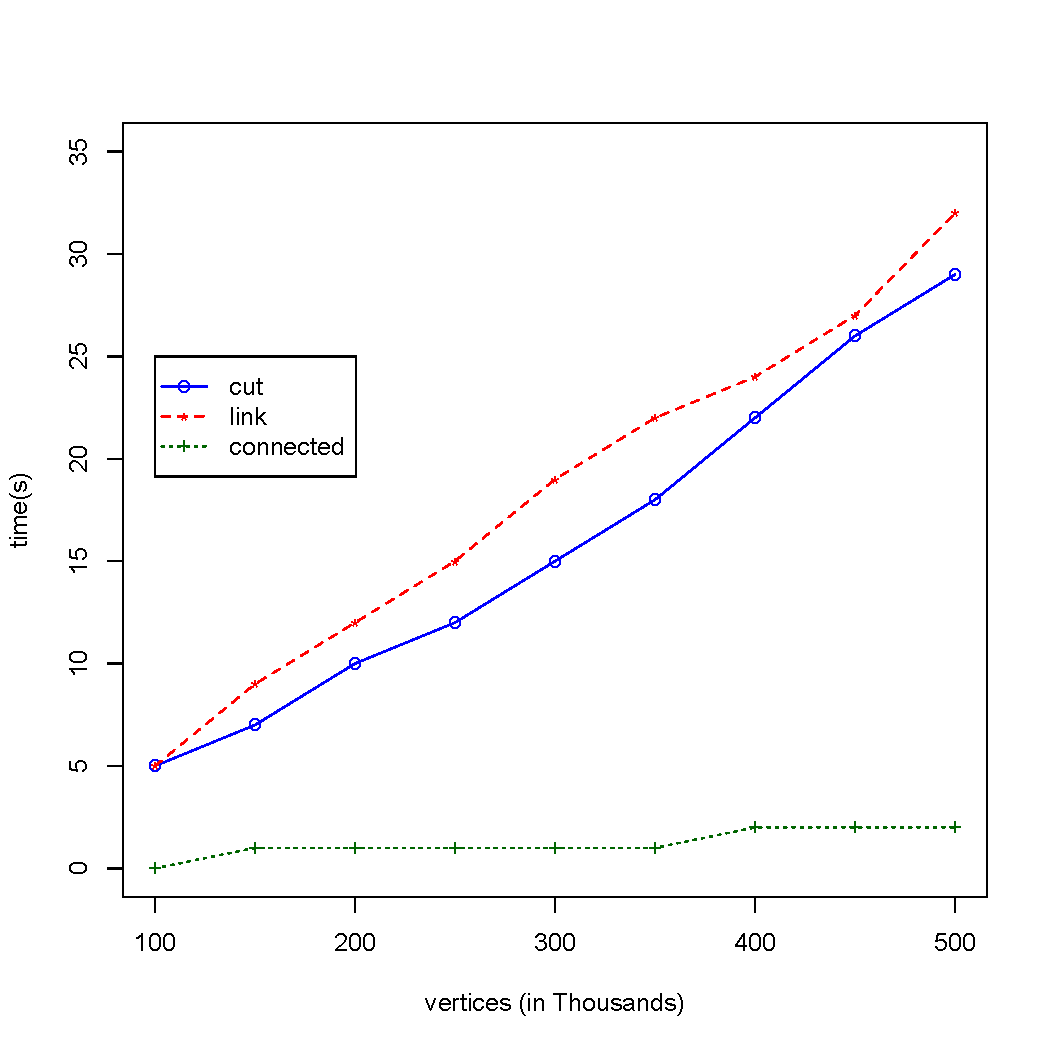
\includegraphics[scale=0.55]{./Images/plot1} 
\end{center}
\caption{Sequence of \textit{link}s, \textit{cut}s, and \textit{connected}s}
\label{fig:plot1}
\end{figure}


\tcb{Deduce regression line in Fig \ref{fig:plot1}}


\textit{Results}. As expected, the growth of the curves by \textit{link} and \textit{cut} is linear. Given a sequence of size $m$ of update operations which take $O(\log n)$ each, the overall time turns into $O(m(\log n))$. This is because every update operation changes the size of the forest which is carry on all the way in the sequence. Finally, \textit{connected}, takes almost constant time, in fact $O(\log n)$, since the size of the forest remains fixed during the sequence. 


\tcr{The introduction promises O(log n) amortised runtimes, but the paper never discusses the amortised aspect. Amortised over what usage? Similarly, the introduction mentions a ``key insight" of O(1) operations, but this train of thought is likewise not picked up later.} 


\tcb{Amortised over what??}


\tcr{Sets in Haskell are trees themselves, and it is odd to store a tree in every node of a tree. Can you take the finger tree, specialized to this particular monoidal annotation, and optimize it further more?}